\documentclass[12pt,a4paper]{cibb}

\usepackage{subfigure,graphicx}
\usepackage{amsmath,amsfonts,latexsym,amssymb,euscript,xr}
\usepackage{caption}

% Package to generate and customize Algorithm as per ACM style
\usepackage[ruled, linesnumbered, noend]{algorithm2e}
\renewcommand{\algorithmcfname}{Listing}
\SetAlFnt{\small}
\SetAlCapFnt{\small}
\SetAlCapNameFnt{\small}
\SetAlCapHSkip{0pt}
\IncMargin{-\parindent}


\title{\large $\ $\\ \bf AUTHOR'S GUIDELINES FOR CIBB PAPERS}

\author{ First Author$^{(1)}$, Second Author$^{(2)}$}
\address{$\ $\\(1) First Institute\\
 Affiliation, address, email
\\
%
\bigskip
(2) Second Institute\\
Affiliation, address, email
}


\abstract{keyword1, keyword2, keyword3, keyword4, keyword5.
\\[17pt]
{\bf Abstract.} Abstract is abstract. Abstract is abstract. Abstract is abstract. Abstract is abstract. Abstract is abstract. Abstract is abstract. Abstract is abstract. Abstract is abstract. Abstract is abstract. Abstract is abstract. Abstract is abstract. Abstract is abstract. Abstract is abstract. Abstract is abstract. Abstract is abstract. Abstract is abstract. Abstract is abstract. Abstract is abstract. Abstract is abstract. Abstract is abstract. Abstract is abstract. Abstract is abstract. Abstract is abstract. }

\begin{document}
\thispagestyle{myheadings}
\pagestyle{myheadings}
\markright{\tt Proceedings of CIBB 2019}%check year

\section{\bf Formal languges}

In this section we introduce some basic definitions from the formal language theory, and describe Valiant's parsing algorithm on which we base our solution.

An alphabet $\Sigma$ is a finite nonempty set of symbols.
$\Sigma^{*}$ is a set of all finite strings over $\Sigma$.
A contex-free grammar $G_S$ is a quadruple $(\Sigma, N, R, S)$, where $\Sigma$ is a finite set of terminals, $N$ is a finite set of nonterminals, $R$ is a finite set of productions of the form $A \rightarrow \beta$, where $\Sigma \cap N = \varnothing$, $A \in N, \beta \in V^{*}$, $V = \Sigma \cup N$ and $S \in N$ is a start symbol.
Context-free grammar $G_S = (\Sigma, N, R, S)$ is said to be in Chomsky normal form if all productions in $R$ are of the form: $A \rightarrow BC$, $A \rightarrow a$, or $S \rightarrow \varepsilon$, where $A, B, C \in N, a \in \Sigma, \varepsilon$ is an empty string.
For each context-free grammar $G$ of length $N$ we can find an equivalent grammar in Chomsky normal form with length $N^2$ ~\cite{hopcroft2008introduction}.

$L_{G}(S) = \{ \omega | S\xrightarrow[G_S]{*} \omega\}$ is a language specified by the grammar $G_{S} = (\Sigma, N, R, S)$, where $A \xrightarrow[G_S]{*} \omega$ means that $\omega$ can be derived in a finite number of rules applications from the start symbol $S$.

\subsection{\bf \it Valiant's parsing algorithm}

Tabular parsing algorithms construct a matrix $T$, cells of which are filled with nonterminals from which the corresponding substring can be derived. 
These algorithms usually work with the grammar in Chomsky normal form.
For $G_S=(\Sigma, N, R, S)$, $T_{i, j} =  \{ A | A \in N, a_{i + 1} \dots a_{j} \in L_{G}(A)\} \quad \forall i < j$.

The elements of $T$ are filled successively starting with $T_{i - 1, i} = \{ A | A \rightarrow a_{i} \in R\}.$
Then, $T_{i, j} = f(P_{i, j}),$ where
$P_{i, j} = \bigcup\limits_{k = i + 1}^{j - 1} T_{i,k} \times T_{k, j}$ and
$f(P) = \{A | \exists A \rightarrow BC \in R : (B, C) \in P\}.$
Finally, the input string $a_{1}a_{2} \dots a_{n}$ belongs to $L_{G}(S)$ iff $S \in T_{0, n}$.

If all cells are filled sequentially, the time complexity of this algorithm is $O(n^3)$.
Valiant proposed to offload the most intensive computations to the Boolean matrix multiplication. 
As the most time-consuming is computing $\bigcup\limits_{k = i + 1}^{j - 1} T_{i, k} \times T_{k, j}$, Valiant's idea is to compute $T_{i, j}$ by multiplication of submatrices of $T$.
Multiplication of two submatrices of parsing table $T$ is defined as follows.
Let $X \in (2^N)^{m \times l}$ and $Y \in (2^N)^{l \times n}$ be two submatrices of the parsing table $T$. 
Then, $X \times Y = Z$, where $Z \in (2^{N \times N})^{m \times n}$ and $Z_{i, j} = \bigcup\limits_{k = 1}^{l} X_{i, k} \times Y_{k, j}$.

Note that the computation of $X \times Y$  can be replaced by the multiplication of $|N|^2$ Boolean matrices (for each nonterminal pair).
Denote the matrix corresponding to the pair $(B, C) \in N \times N$ as $Z^{(B, C)}$, then $Z_{i, j}^{(B, C)} = 1$ iff $(B, C) \in Z_{i, j}$.
It should also be noted that $Z^{(B, C)} = X^{B} \times Y^{C}$.
Each Boolean matrix multiplication can be computed independently.
Following these changes, time complexity of this algorithm is $O(|G|\mathrm{BMM}(n)log(n))$ for an input string of length $n$, where $\mathrm{BMM}(n)$ is the number of operations needed to multiply two Boolean matrices of size $n \times n$.

Valiant's algorithm written as proposed by Okhotin is presented in Listing~\ref{algo:valiant}.
All elements of $T$ and $P$ are initialized by empty sets.
Then, the elements of these two table are successively filled by two recursive procedures.

% Algorithm1
\begin{algorithm}[h]
\SetAlgoNoLine
\KwIn{Grammar $G = (\Sigma, N, R, S), w = a_{1} \dots a_{n}, n \geq 1, a_{i} \in \Sigma$, where  $n + 1 = 2^k$}
\underline{main()}{:}{

 \textit{compute(0, n + 1)\;}
 accept if and only if $S \in T_{0, n}$
 \linebreak
 }

\underline{compute(\textit{l, m})}{:}{

 \If {$m - l \geq 4$}{
     \textit{compute(l, $\frac{l+m}{2}$)\;
     compute($\frac{l+m}{2}$, m)}}
 \textit{complete(l, $\frac{l+m}{2}$, $\frac{l+m}{2}$, m)}
 \linebreak
 }

\underline{complete(\textit{l, m}, $l^\prime$, $m^\prime$)}{:}{

 \lIf {$m - l = 4$ and $m = l^\prime$}{$T_{l, l + 1} = \{A | A \rightarrow a_{l+ 1} \in R\}$}
 \lElseIf{$m - l = 1$ and $m < l^\prime$}{ $T_{l, l'} = f(P_{l, l'})$}
 \ElseIf{$m - l > 1$}{
    $\textit{leftgrounded} = (l, \frac{l+m}{2}, \frac{l+m}{2}, m), \textit{rightgrounded} = (l', \frac{l'+m'}{2}, \frac{l'+m'}{2}, m')$,

    $\textit{bottom} = (\frac{l+m}{2}, m, l', \frac{l'+m'}{2}), left = (l, \frac{l+m}{2}, l', \frac{l'+m'}{2})$,

    $\textit{right} = (\frac{l+m}{2}, m, \frac{l'+m'}{2}, m'), top = (l, \frac{l+m}{2}, \frac{l'+m'}{2}, m')$\;
    \textit{complete(bottom)}\;
    $P_{\textit{left}} = P_{\textit{left}} \cup (T_{\textit{leftgrounded}} \times T_{\textit{bottom}})$\;
    \textit{complete(left)}\;
    $P_{\textit{right}} = P_{\textit{right}} \cup (T_{\textit{bottom}} \times T_{\textit{rightgrounded}})$\;
    \textit{complete(right)}\;
    $P_{\textit{top}} = P_{\textit{top}} \cup (T_{\textit{leftgrounded}} \times T_{\textit{right}})$\;
    $P_{\textit{top}} = P_{\textit{top}} \cup (T_{\textit{left}} \times T_{\textit{rightgrounded}})$\;
    \textit{complete(top)}
    }
 }
\caption{Parsing by Matrix Multiplication: Valiant's Version}
\label{algo:valiant}
\end{algorithm}

The procedure $compute(l, m)$ computes correct values of $T_{i,j}$ for all $l \le i < j < m$.

The procedure $complete(l, m, l', m')$ constructs the submatrix $T_{i, j}$ for all $l \le i < m$, $l' \le j < m'$. This procedure assumes $T_{i, j}$ for all $l \leq i < j < m,  l' \leq i < j < m'$ are already constructed and the current value of  $P_{i, j} =  \{ (B, C) |\exists k, (m \le k < l'), a_{i + 1} \dots a_{k} \in L(B), a_{k + 1} \dots a_{j} \in L(C)\}$ for all $l \leq i < m,  l' \leq j < m'$.
The submatrix partition during the procedure call is shown in Figure~\ref{fig1}.


\begin{figure}
\vspace{3mm}
 \begin{center}
    \begin{minipage}{0.48\textwidth}
        \centering
        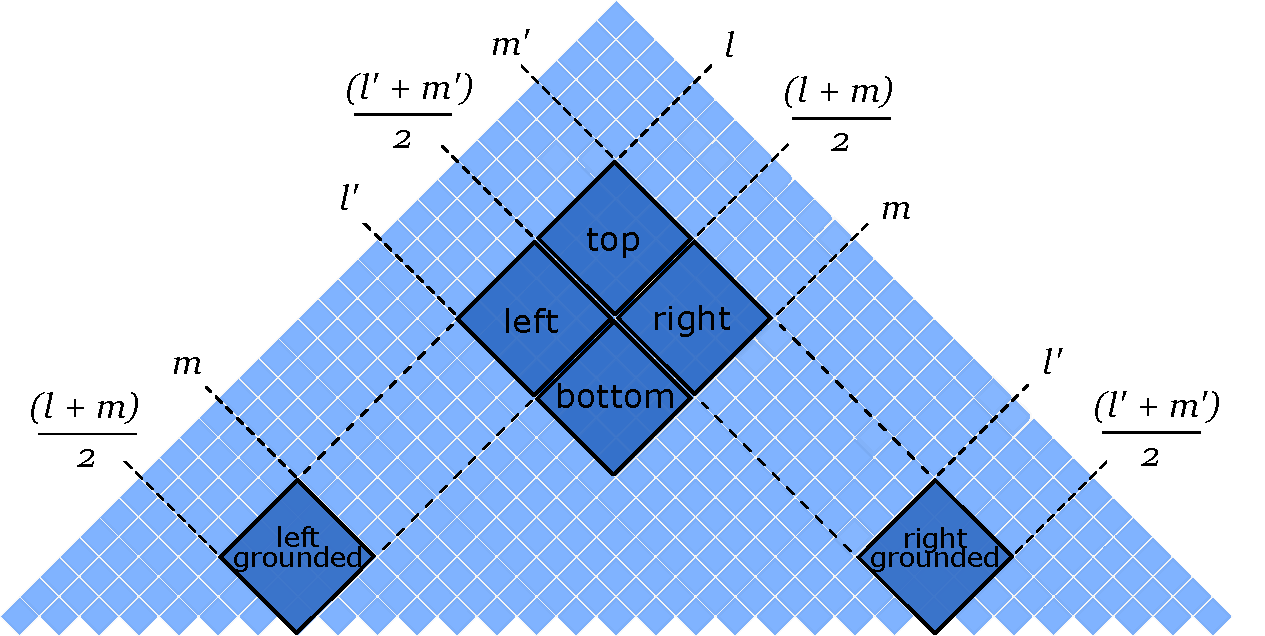
\includegraphics[width=6cm]{pictures/splitting_with_grounded.pdf}
        \caption{Matrix partition used in procedure \textit{complete(l, m, l', m')}}
        \label{fig1}
    \end{minipage}\hfill
    \begin{minipage}{0.48\textwidth}
        \centering
        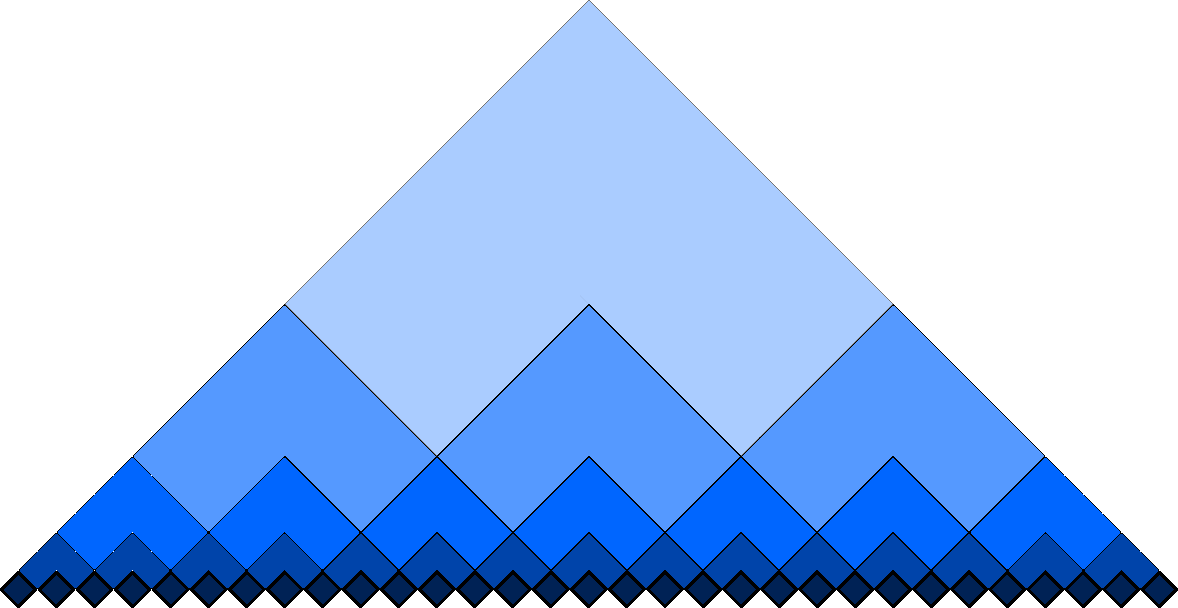
\includegraphics[width=6cm]{pictures/layers.pdf}
        \caption{Matrix partition on V-shaped layers used in modification}
        \label{fig2}
    \end{minipage}
 \end{center}
\vspace{-8mm}
\end{figure}

A simple example of parsing with the Valiant's algorithm is presented in Figure~\ref{fig3}.
Only several steps are shown, but it is enough to compare our version with the original algorithm.

\begin{figure}
\vspace{3mm}
 \begin{center}
 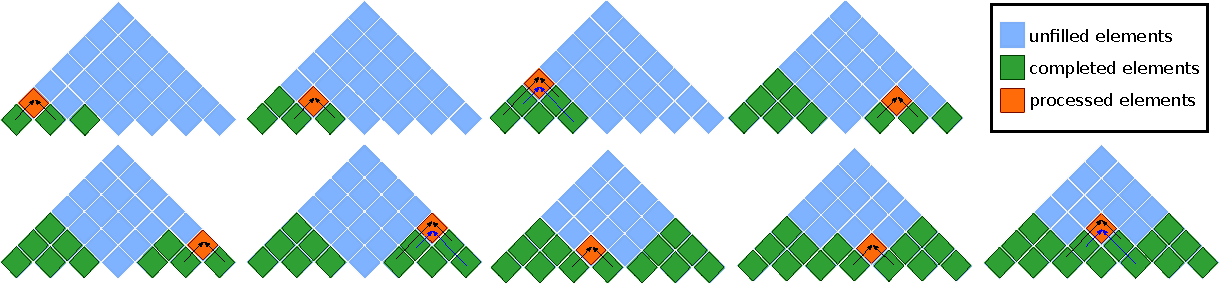
\includegraphics[width=12cm]{pictures/valbeg2.pdf}
    \caption{An example of beginning of Valiant's algorithm}
    \label{fig3}
\end{center}
\vspace{-8mm}
\end{figure}
\section{\bf Modified Valiant's algorithm}

In this section we describe the reorganization of submatrix processing order in the Valiant's algorithm which simplify independent handling of submatrices. As a result, proposed modification can facilitate implementation of parallel submatrix processing.

\subsection{\bf \it New approach}

The main change of this modification is the possibility to divide the parsing table into layers of disjoint submatrices of the same size.
The idea of division we have made from the reorganization of the matrix multiplication order is presented in figure~\ref{fig2}.
Each layer consists of square matrices which size is power of 2.
The layers are computed successively in the bottom-up order.
Each matrix in the layer can be handled independently, which can help to implement parallel version of layer processing function.

\begin{figure}[h]
\vspace{3mm}
 \begin{center}
 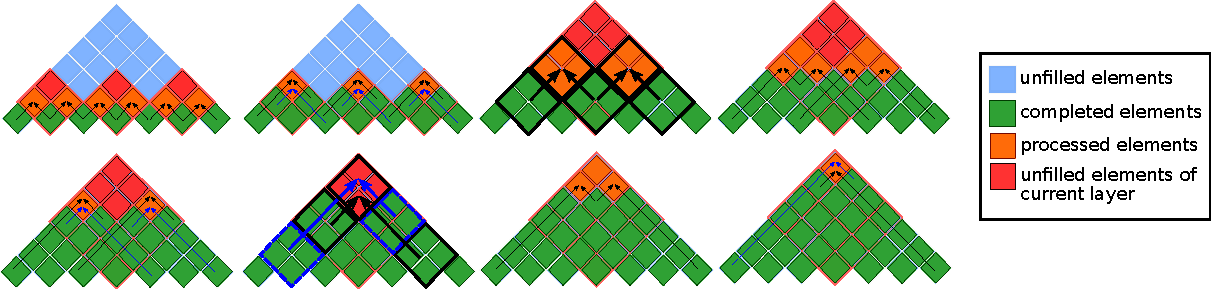
\includegraphics[width=12cm]{pictures/modivis2.pdf}
    \caption{An example of the modification of Valiant's algorithm}
    \label{fig4}
 \end{center}
\vspace{-8mm}
\end{figure}

A simple example of the modification is shown in figure~\ref{fig4}.
The lowest layer (submatrices which size is 1) is already computed and filling of the matrix starts with the second layer (subfigures 1-2).
Note that the same  process is presented in figure~\ref{fig3}, but here it can be done only in two steps using parallel computation of submatrix products.

The modified version of Valiant's algorithm is presented in listing~\ref{algo:modified}.
The procedure \textit{main()} computes the lowest layer $(T_{l, l+1})$, and then divide the table into layers, described earlier, and computes them through the \textit{completeVLayer()} call.
Thus, \textit{main()} computes all elements of parsing table $T$.
(Hereinafter, we use layer to mean set of submatrices.)

For brevity, we define \textit{left(subm), right(subm), top(subm), bottom(subm), \linebreak rightgrounded(subm)} and \textit{leftgrounded(subm)} functions which returns the submatrices for matrix $subm = (l, m, l', m')$ according to the original Valiant's algorithm (figure~\ref{fig2}).

Also denote some subsidiary functions for matrix layer $M$:
\begin{itemize}[noitemsep, nolistsep]
    \item[$-$] \textit{bottomsublayer(M)} $ = \{bottom(subm)\, |\,subm \in M \}$,
    \item[$-$] \textit{leftsublayer(M)} $ = \{\textit{left(subm)}\, |\,subm \in M \}$,
    \item[$-$] \textit{rightsublayer(M)} $ =\{\textit{right(subm)}\, |\,subm \in M \}$,
    \item[$-$] \textit{topsublayer(M)} $ = \{top(subm)\, |\,subm \in M \}$.
\end{itemize}

\begin{algorithm}[!h]
\SetAlgoNoLine
\KwIn{$G = (\Sigma, N, R, S), w = a_{1} \dots a_{n}, n \geq 1, n + 1 = 2^p, a_{i} \in \Sigma$ }
\underline{main()}{:}{

 \For {$l \in \{1, \ldots, n \}$}{$T_{l, l + 1} = \{A | A \rightarrow a_{l + 1} \in R\}$}
 \For{$1 \le i < p - 1 $}{
 layer = \textit{constructLayer(i)}\;
 \textit{completeVLayer(layer)}
 }
 accept if and only if $S \in T_{0, n}$
 \BlankLine
 }

\underline{constructLayer(i)}{:}{
 \BlankLine
 $\{(k2^i, (k+1)2^i, (k + 1)2^i, (k+2)2^i) \, |\, 0 \le k < 2^{p - i} - 1\}$
 \BlankLine
    }
\underline{completeLayer(M)}{:}{
\BlankLine
\If {$\forall (l, m, l', m') \in M \quad (m - l = 1)$}{\For{$ (l, m, l', m') \in M$}{$T_{l, l'} = f(P_{l, l'})$\;}}
\Else{
\textit{completeLayer(bottomsublayer(M))}\;
\textit{completeVLayer(M)}
}
\BlankLine
}

\underline{comleteVLayer(M)}{:}{
 \BlankLine
 \textit{multiplicationTasks$_1$ = \linebreak
    \{$left(subm)$, $leftgrounded(subm)$, $bottom(subm)\, |\,subm \in M \} \cup \linebreak  \{right(subm), bottom(subm), rightgrounded(subm)\, |\,subm \in M\}$\;}
 \BlankLine
 multiplicationTask$_2$ = $\{top(subm), leftgrounded(subm), right(subm)\, |\,subm \in M\}$\;
 \BlankLine
 multiplicationTask$_3$ = $\{top(subm), left(subm), rightgrounded\, |\,subm \in M\}$\;
 \BlankLine
 \textit{performMultiplications(multiplicationTask$_1$)}\;
 \textit{completeLayer(leftsublayer(M) $\cup$ rightsublayer(M))}\;
 \textit{performMultiplications(multiplicationTask$_2$)}\;
 \textit{performMultiplications(multiplicationTask$_3$)}\;
 \textit{completeLayer(topsublayer(M))}

 }
 \BlankLine

 \underline{performMultiplication(tasks)}{:}{\\
 \For{$ (m, m1, m2) \in \textit{tasks}$}{$P_{m} = P_{m} \cup (T_{m1} \times T_{m2})$\;}
 }

\caption{Parsing by matrix multiplication: Modified Version}
\label{algo:modified}
\end{algorithm}


The procedure \textit{completeVLayer(M)} takes an array of disjoint submatrices $M$ which represents a layer.
For each \textit{subm = (l, m, l', m') $\in M$} this procedure computes \textit{left(subm), right(subm), top(subm)}.
The procedure assumes that the elements of \textit{bottom(subm)} and $T_{i, j}$ for all $i$ and $j$ such that $l \leq i < j < m$ and $  l' \leq i < j < m'$ are already constructed.
Also it is assumed that the current value of
$P_{i, j} =  \{ (B, C) | \exists k, (m \le k < l'), a_{i + 1} \dots a_{k} \in L_G(B), a_{k + 1} \dots a_{j} \in L_G(C)\} $ for all $i$ and $j$ such that $l \leq i < m$ and $l' \leq j < m'$.

The procedure \textit{completeLayer(M)} also takes an array of disjoint submatrices $M$, but unlike the previous one, it computes $T_{i, j}$ for all $(i, j) \in subm$.
This procedure requires exactly same assumptions on $T_{i, j}$  and $P_{i, j}$  as in the previous case.

In the other words, \textit{completeVLayer(M)} computes the entire layer \textit{M} \linebreak and \textit{completeLayer($M_{2}$)} is a support function which is necessary for computation of smaller square submatrices $subm_{2} \in M_{2}$ inside of \textit{M}.

Finally, the procedure \textit{performMultiplication(tasks)}, where \textit{tasks} is an array of a triple of submatrices, perform basic step of algorithm: matrix multiplication. It is worth mentioning that, as distinct from the original algorithm, here $|tasks| \ge 1$ and each task can be computed independently.
So, practical implementation of this procedure can easily involve different techniques of parallel array processing, such as OpenMP~\ref{!!!}.

\subsection{\bf \it Algorithm for substrings}

Next we show how our modification can be applied to the string-matching problem.

So if we want to find all substrings of size $s$ which can be derived from a start symbol for an input string of size $n = 2^p$, we need to compute layers with submatrices of size not greater than $2^{l'}$, where $2^{l' - 2} < s \le 2^{l' - 1}$.

Let $l' = p - (m - 2)$ and consequently $(m - 2) = p - l'$.

For any  $m \le i \le p$ products of submatrices of size $2^{p - i}$ are calculated exactly $2^{2i - 1} - 2^{i}$ times and each of them imply multiplying $\mathcal{O}(|G|)$ Boolean submatrices.

\begin{equation}
\begin{array}{c}
C \sum\limits_{i=m}^p 2^{2i - 1} \cdot 2^{\omega(p - i)} \cdot f(2^{p - i}) =
C \cdot 2^{\omega l'}\sum\limits_{i=2}^{l'} 2^{(2 - \omega)i} \cdot 2^{2(p - l') - 1} \cdot f(2^{l' - i}) \le \\
C \cdot 2^{\omega l'} f(2^{l'}) \cdot 2^{2(p - l') - 1} \sum\limits_{i=2}^{l'} 2^{(2 - \omega)i} =
BMM(2^{l'}) \cdot 2^{2(p - l') - 1} \sum\limits_{i=2}^{l'} 2^{(2 - \omega)i}
\end{array}
\end{equation}

Thus, time complexity for searching all substrings is  $O(|G|BMM(2^{l'})(l' - 1))$, while time complexity for the full input string is $O(|G|BMM(2^p)(p - 1))$. In contract to the modification, Valiant's algorithm completely calculate at least 2 triangle submatrices of size $\frac{n}{2}$ (as shown in figure~\ref{fig5}) which mean minimum asymptotic complexity  $O(|G|BMM(2^{p - 1})(p - 2))$. Make a conclusion that the modification is asymptotically faster for substrings of size $s \ll n$  than the original algorithm.

\begin{figure}[h]
\vspace{3mm}
 \begin{center}
 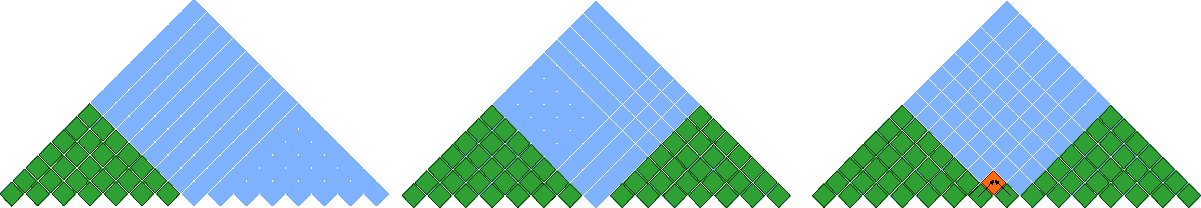
\includegraphics[width=12cm]{pictures/valsubstring.pdf}
    \caption{The number of elements necessary to compute in Valiant's algorithm. That means it is nessesary to calculate at least 2 triangle submatrices of size $\frac{n}{2}$.}
    \label{fig5}
 \end{center}
\vspace{-8mm}
\end{figure}

\section{Conclusion and future work}
In this paper, we shown how the context-free path query evaluation w.r.t. the relational and the single-path query semantics can be reduced to the calculation of matrix transitive closure. Also, we provided a formal proof of the correctness of the proposed reduction. In addition, we introduced an algorithm for computing this transitive closure, which allows us to efficiently apply GPGPU computing techniques. Finally, we shown the practical applicability of the proposed algorithm by running different implementations of our algorithm on real-world data.

We can identify several open problems for further research. In this paper we have considered only two semantics of context-free path querying but there are other important semantics, such as all-path query semantics~\cite{hellingsPathQuerying} which requires to present all paths for all triples $(A,m,n)$. Context-free path querying implemented with algorithm~\cite{GLL} can answer the queries in all-path query semantics by constructing a parse forest. It is possible to construct a parse forest for a linear input by matrix multiplication~\cite{okhotin_cyk}. Whether it is possible to generalize this approach for a graph input is an open question.

In our algorithm, we calculate the matrix transitive closure naively, but there are algorithms for the transitive closure calculation, which are asymptotically more efficient. Therefore, the question is whether it is possible to apply these algorithms for the matrix transitive closure calculation to the problem of context-free path querying.

Also, there are Boolean grammars~\cite{okhotinBoolean}, which have more expressive power than context-free grammars. Boolean path querying is an undecidable problem~\cite{hellingsRelational} but our algorithm can be trivially generalized to work on boolean grammars because parsing with boolean grammars can be expressed by matrix multiplication~\cite{okhotin_cyk}. It is not clear what a result of our algorithm applied to Boolean grammars would look like. Our hypothesis is that it would produce the upper approximation of a solution.

From a practical point of view, matrix multiplication in the main loop of the proposed algorithm may be performed on different GPGPU independently. It can help to utilize the power of multi-GPU systems and increase the performance of context-free path querying.

There is an algorithm~\cite{apspGPU} for transitive closure calculation on directed graphs which generalized to handle graph sizes inherently larger then the DRAM memory available on the GPU. Therefore, the question is whether it is possible to apply this approach to the matrix transitive closure calculation in the problem of context-free path querying.


\section*{\bf Acknowledgments}

Example of the Acknowledgments section.



\bibliographystyle{apalike}
{\fontsize{10}{10}\selectfont
\begin{thebibliography}{99}
\setlength{\parskip}{0pt}


\end{thebibliography}
}

\end{document}



